\documentclass[a4paper,12pt,twoside]{article}
\usepackage[T1]{fontenc}
\usepackage[utf8]{inputenc}
\usepackage{lmodern}
\usepackage{url,csquotes}
\usepackage[hidelinks,hyperfootnotes=false]{hyperref}
\usepackage[titlepage,pagenumber]{polytechnique}
\usepackage{float}

\title{MAP-536 - Python for Data Science}
\subtitle{Final Project - Air data prediction}
\author{Leonardo \textsc{Natale} \& Guillaume \textsc{Le Fur}}
\logo{scikit_learn.jpeg}

\begin{document}

\maketitle

\section{External Data and Data Preprocessing}

\subsection{Getting External Data}

The original data consists of : 

\begin{table}[H]
	\centering
	\begin{tabular}{|l|l|}
	\hline
	\textbf{Feature} & \textbf{Description}                          \\ \hline
	DateOfDeparture  & Date of departure                             \\ \hline
	Departure/Arrival& Departure and arrival airport                 \\ \hline
	WeeksToDeparture & Average number of weeks before departure when the ticket is booked \\ \hline
	log\_PAX          & Variable related to the number of passengers \\ \hline
	std\_wtd          & Standard deviation of WeeksToDeparture       \\ \hline
	\end{tabular}
\end{table}

We have added the following data:

\begin{table}[H]
	\centering
	\begin{tabular}{|l|l|}
	\hline
	\textbf{Feature} & \textbf{Description}                        \\ \hline
	jet\_fuel        & Daily jet fuel price                        \\ \hline
	coordinates      & Airport geographical coordinates            \\ \hline
	gdp              & Departure and Arrival GDP                   \\ \hline
	passengers       & Monthly flow of passengers between airports \\ \hline
	holiday          & holiday data is the U.S.                    \\ \hline
	\end{tabular}
\end{table}

\subsection{Feature Engineering}

We were able to add the following extra features, by using the data described above:
\begin{itemize}
	\item Number of days to the closest holiday.
	\item Distance in kilometers between departure and arrival airport.
	\item Airport Dimension
	\item Monthly log\_PAX per airport, both arrival and departure.
\end{itemize}


\section{Structure}
(Adjust the size and position, maybe explanation at the right)

\begin{figure}[H]
	\centering
	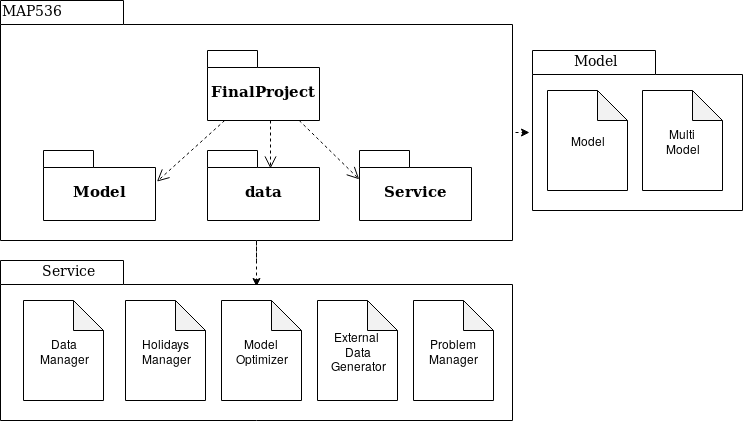
\includegraphics[scale=0.5]{UML.png}
\end{figure}

\begin{itemize}
	\item \textbf{Data} contains all the external data files that we use to create our additional features.
	\item \textbf{ExtrnalDataGenerator} merges all our external data into the \textit{external\_data.csv} file. It is the class that is responsible for all the feature engineering of our models.
	\item \textbf{DataManager} is some kind of an interface between the model and the external data. It takes data as an input (either the train or test data) and merges it with external data, making it ready for fitting.
	\item \textbf{Model} is a utility class that stores a sklearn model and two lists : a list of parameters that are to optimize via GridSearchCV and another with parameters that are to be optimized via RandomSearchCV. The main role of this class, when used locally, is to compare the quality of the fit of a model before and after optimization of the hyper-parameters. When used on RAMP, it's role is to contain the model and to fit and predict based on the data passed as an input.
	\item \textbf{MultiModel} is a class that goal is to simplify the testing of multiple models at the same time. When creating an instance, one can pass multiple models and hyper-parameters list. Then all the models are going to be optimized. The predict method can be used in two different ways : either returning separate predictions for each model or either making the average of the models, which can allow to test models that are combinations of several models.
	\item \textbf{ModelOptimizer} is an interface, called by Model, that takes care of the RandomSearchCV and GridSearchCV and returns the result to model.
	\item \textbf{HolidaysManager} is a utility class used to vectorize operations on dates to determine whether they are holidays or how close they are to a holiday.
	\item \textbf{ProblemManager} is a class that contains metadata about the problem we intend to solve (columns that are relevant, external data we use, etc.)
\end{itemize}

\section{Models and Tuning}
\subsection{Models}
Add a table with comparison between different models.
\begin{center}
	\begin{tabular}{| c | c | c | c |} 
		\hline
			 & Train RMSE & Test RMSE & Train time (s) \\ [0.5ex] 
		\hline
		\textbf{RandomForest} & 0.62 & 0.81 & 5.6 \\ 
		\hline
		\textbf{GradientBoostingRegressor} & 0.40 & 0.52 & 7.67 \\
		\hline
		\textbf{HistGradientBoostingRegressor} & \textbf{0.27} & \textbf{0.37} & \textbf{5.18} \\
		\hline
		\textbf{HistGradientBoostingRegressor (Tuned)} & 0.11 & 0.35 & 11.8 \\
		\hline
		\textbf{AdaBoostRegressor} & 0.19 & 0.34 & 107 \\
		\hline
	\end{tabular}
\end{center}

The Model we chose in the end is \textbf{HistGradientBoostingRegressor}, mostly because it's a good compromise between accuracy and training time. It's also the model that gives the best results without overfitting too much. Indeed, after a certain point ($RMSE_{test} \approx 0.37$), making the RMSE better by tuning hyper-parameters resulted in a very low training error ($RMSE_{train} \approx 0.07$).


\subsection{Hyper-parameter Tuning vs Feature Importance}

During the project, we tried several models, made some hyper-parameter tuning and also added features along the way. We thought it would be interesting to keep track of the evolution of the value of our RMSE over time.
The following graphs displays the evolution of our RMSE over time, along with the reasons of the main changes.

\begin{figure}[H]
	\centering
	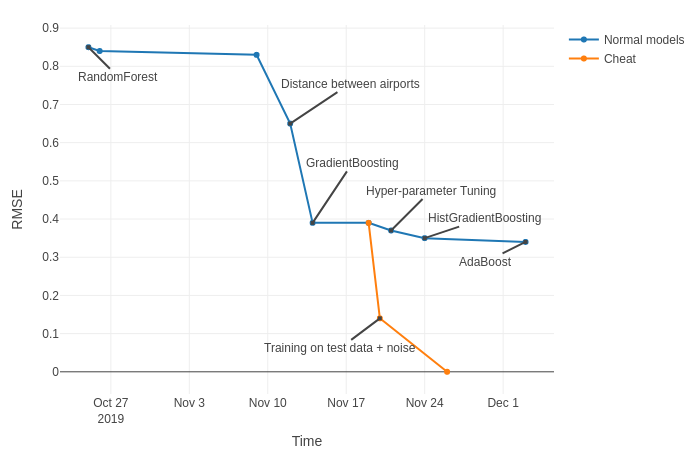
\includegraphics[scale=0.5]{rmse_evolution.png}
\end{figure}

What we can see is that the main changes were due to adding new features to our data, rather than optimizing the hyper-parameters, which often led to overfitting.

\section{Conclusion}

\subsection{Model Interpretability}

\begin{figure}[H]
	\centering
	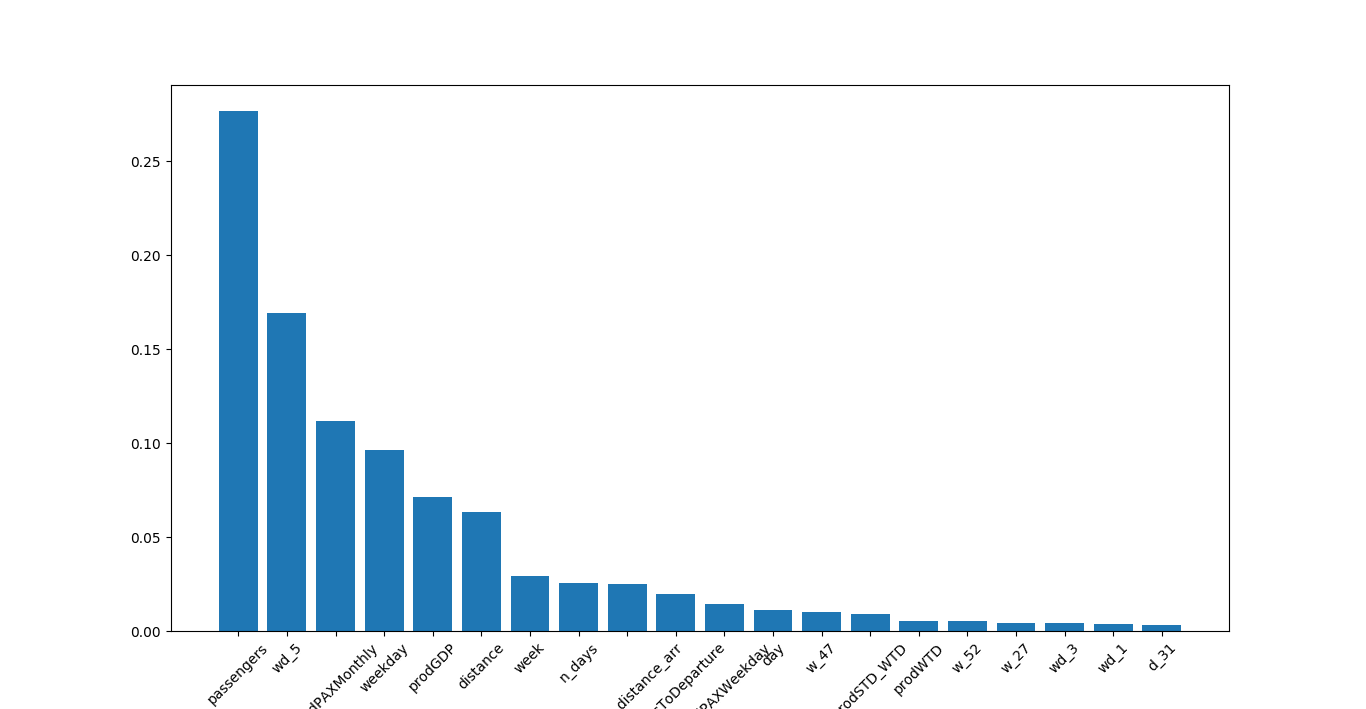
\includegraphics[scale=0.5]{feature_importance.png}
\end{figure}

Feature importance graph and comments.

\subsection{Evaluation of Uncertainty in Predictions}

Because we don't have much data, we cannot say that our predictions are extremely accurate. It's all the more problematic that the values of log\_PAX are not spread a lot (mostly between 9 and 12)

\subsection{Final Comments and Possible Improvements}

We didn't have time to try the time series but it would have been interesting to fit a time series on the biggest Departure airports to see how it performed on such data.

\end{document}
